\chapter{Eclipse Modeling Framework (EMF)}
"EMF is a Java framework and code generation facility for building tools and other applications based on a structured (data) model" \cite{EMFDoc}
 It unifies three important technologies: a subset of Java, XML and a subset of UML. Models are definable by an XML Schema, annotated Java interfaces or by UML modeling tools. EMF bridges the gap between modelers and Java programmers by relating modeling concepts to a simple Java representation of these concepts. \cite{EMF2nd}\\

EMFs runtime framework allows data to be validates, persisted and edited in a UI Editor. Change recording and notification as well as metadata by reflection is available. EMF is the foundation for fine-grained interoperability and data sharing among tools. For example 
\todo{Mention base for transactions, graphical editors, DB persistence, M-trans}\\ \todo{Mention runtime instances?}\\

EMF supports saving models to and loading them from persistent resources. A default XMI, a specialized XML, serialization is available as a default serialization format. References can be persisted, they can be across multiple resources, with load on demand, proxy resolution, unloading support. References can be bidirectional in EMF with referential integrity maintained. \cite{EMF2nd}\\

\section{Ecore Meta Model}
EMF uses a model to describe other EMF models. This model is called Ecore and is the center of the EMF world. Ecore is itself an EMF model and can be described by itself similar to the possibility of describing the syntax of EBNF in EBNF. This makes Ecore its own metamodel, thus Ecore is a meta-metamodel. The concepts of metamodels is simple: a model which describes a model is a metamodel. A model which describes a metamodel is a meta-metamodel. \cite{EMF2nd}  A metamodel describes the abstract syntax of a language \cite{EMP} and the added validation rules the static semantics of a language \cite{MDSD}

Ecore supports several high level concepts which are not directly available in Java, like bidirectional relationships, and a specialization of it, containment relationships.

	\todo{Cycles in composition are not allowed; composition forms trees within models. The roots of these trees are model elements without container; the leafs are elements without components.}
	


The following describes a subset of Ecore, based on \cite{EMF2nd} \\

\todo{BILD!}


\begin{itemize}
	\item An EPackage is the root of an model and contains EClassifiers and sub packages.
	\item EClasses models classes. A class refers a number of other classes as its super types. They are identified by name and contains a number of attributes and references which both are structural features.
	\item EStructuralFeature is the super type of attributes and references aggregates attributes like multiplicity.
	\item EAttributes have a type and are identified by name. They model the components of an objects data.
	\item EDataType represents a single type which must not impose structure. They are directly related to Java types.
	\item EClass and EData types are both EClassifiers.
	\item EReferences model one end of an association. They are identified by name and hold a type of the referable object. If the association is bidirectional, the eOpposite is assigned to its inverse reference. \cite{EMF2nd}
	\item ECore classes hold and eAnnotation reference. Annotations store information which were not considered fundamental enough to explicitly support them in Ecores metamodel. For example documentation, OCL validation, XML serialization parameters. \cite{EMP}
	\item In additional to structural features, Ecore can also model the interfaces of behavioral features.
\end{itemize}

\section{Generator model}
The generator model is the model that provides access to the data needed to generate the Ecore model by decorating it. This separation has the advantage that the Ecore model can remain pure without code generation dependent information with the disadvantage that it might get out of sync. \cite{EMF2nd}

\section{MOF vs Ecore}
Meta-Object Facility (MOF) is a modeling concept comparable to Ecore. It is defined by the Object Management Group \cite{OMG} to define UML2. Essential Meta-Object Facility (EMOF) is the lightweight core of MOF that closely resembles Ecore. EMF can read and write EMOFs serialization format. \cite{EMP}

\section{Runtime}
EMFs runtime framework provides the basis for manipulation, change notification and serialization of EMF objects in general. \cite{EMF2nd} Change notification is based on the observer pattern, which are called adapters in EMF, because they frequently extend behavior of EObjects and adapt them.

The relevant runtime concepts are EMF.Edit, as an example of an simple editor or controller and persistence, because XText \cite{XTextMan} and EMF.Edit integrate itself in EMF using persistence concepts.

\subsection{Persistence}
Resource, and ResourceSet are fundamental interfaces of EMFs persistence framework.


\subsubsection{Cross Resource References}
To reference other persisted objects, EMF uses Proxies. A Proxy is an uninitialized instance of the target class, which is identified by an URI. " A Uniform Resource Identifier (URI) is a compact sequence of characters that identifies an abstract or physical resource."\cite{URI} A URI consists of five parts: scheme, authority, path, query and fragment whereby query is irrelevant for this thesis. The basic format is\\
\code{schema://authority/path\#fragment} \\
The schema defines the interpretation of the following part. Common schemata for EMF are file, in an eclipse environment platform and http. Authority and path together identify an resource, the fragment identifies a part of an resource or in EMFs case an \code{EObject}.
For example:\\
\code{http://www.xtext.my/MiniJava\#//@class.1}\\
which identifies the the second element stored in the containment reference class of http://www.xtext.my/MiniJava resource.


\subsubsection{Resource}
A resource is a basic unit of persistence. It is a container for one or more objects which are persisted together with their children. They can be unloaded in which case contained referred objects  are converted to proxies. An resource is identified by a URI with schema, authority and path. A resource is also responsible for creating valid URI fragments for EObjects contained in it. By default a resource returns hierarchy based XPath like fragments. Other options are intrinsic IDs and extrinsic IDs. Intrinsic IDs are IDs stored directly on the model object, whereas extrinsic IDs are stored external of the object. Extrinsic IDs are useful when the modeled objects state is not sufficient to constitute an ID for a given resource. XML resources manage extrinsic IDs and offer support for universally unique identifiers (UUIDs). It is possible to attach adapters to a resource, so it is for example possible to observe every change of an contained object and create a \code{ChangeModel} by using EMFs \code{ChangeRecorder}. This enables automatic undo support for commands. \cite{EMF2nd}

\subsubsection{ResourceSet}
A ResourceSet acts as a container for Resources and its main responsibility is to support references between objects in different resources. 

\subsubsection{XML Metadata Interchange (XMI)}
XMI is the standard serialization format of EMF models in XML. The "XMI format (...) could technically be considered a concrete syntax, although it's sometimes called a serialization syntax." \cite{EMP}

\section{EMF.Edit}
With EMF Edit it is possible to build editors for models, which display and edit (i.e. Copy, drag-and-drop, etc.) model instances with unlimited undo and redo. EMF.Edit is the controller in the MVC pattern which uses JFace viewers by default. EMF.Edit and GMF controllers are in between view and model, so the view has no direct connection to the model. EMF.Edit supports object modification based on the Command pattern and includes a number of common commands. A command  offers execute, undo, redo and canExecute to check if all constraints are satisfied.  EMF.Edit includes a set of generic commands based on the reflective API like Set, Add, Remove, Move, Replace and Copy, as well as  higher level commands like CreateChild, DeleteChild, CutToClipboard, CopyToClipboard, PasteFromClipboard and DragAndDrop. Controllers are called ItemProviders im EMF.Edit, they offer to navigate their structure, modify their content, to retrieve labels, to forwards notifications to the viewer as well as acting as a command factory. Controller are in general associated with an EObject, but don't need to, in order to let the editor display a structure different from the models structure. The central unit of EMF.Edit is the EditingDomain which encapsulates a ResourceSet, adds a command stack to support undos and redos as well as provides a controller factory. \cite{EMF2nd} 


\section {Graphical Modeling Framework (GMF)}
GMF is a framework for creating graphical eclipse editors that are based on an EMF model. It's a controller framework using EMF Models for persistence and Draw2D as View. GMF is based on GEF and unifying GEF and EMF commands and extensively uses eclipse extension points. Furthermore it adds a notation model, which persists layout information independent from the language metamodel and model. The concept of a Notation Model is explained in detail and how it is integrated in GMF. The main purpose of GMF, the controller, is skipped because the much simpler controllers of EMF.Edit are sufficient in the context of this thesis. To bridge the gap, it's important to note that GMF creates a controller for each View, that is the basic model element of the notation model. Creating more than one View e.g. by the view service factory is a common practice in GMF to separate the presentation structure from model structure. Which view should be created is hinted by the Extensible Type Registry.

\subsection{Notation Model}
GMFs notation model manages and persists the state of the diagram or view separated from the language model. It is completely domain model independent and thus can be handled generically by GMFs engine to provide common features. It manages the diagram element, position and style attributes. \cite{EMP} The base type of the notation model is View, which:
\begin{itemize}
	\item holds a reference to the language model element it represents 
	\item acts as the super type for node, edge and the notation models root: diagram
	\item contains child nodes and refers to edges
	\item has attributes like visibility and type
\end{itemize}

\begin{center}
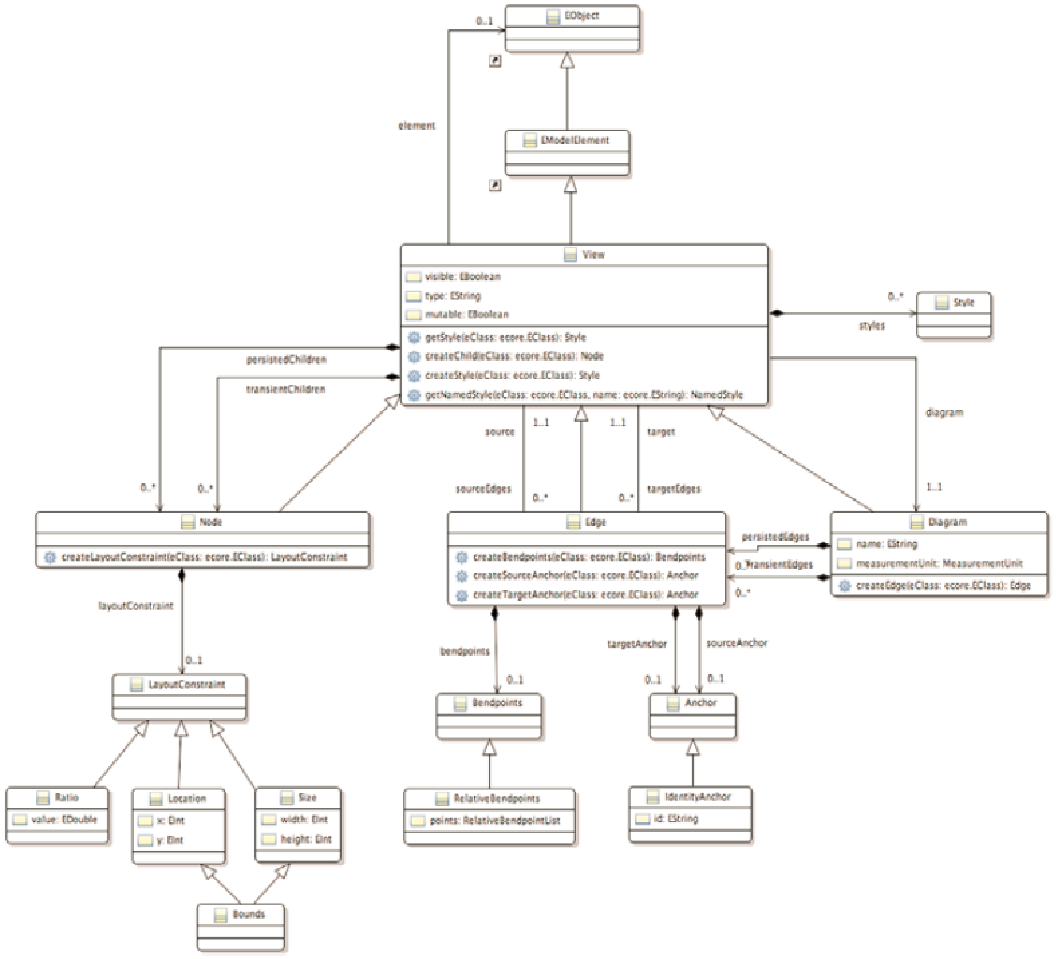
\includegraphics[scale=0.5]{gfx/NotationMM.png}
\end{center}
\todo{Mention EMP}

Part of the design considerations for the notation meta model were \cite{GMFDoc}:
\begin{itemize}
	\item The notation meta-model was designed to minimize merging conflicts through the separation of style into granular properties. They can be merged independently.
	\item The style hierarchy has been designed to be extend able. The allows individual extensions and enhancements in the future. 
\end{itemize}

\subsection{View Service}
The View Service is a factory for constructing new notation view elements also based on \cite{GMFDoc}:
\begin{itemize}
	\item the corresponding language element (EObject)
	\item the type determined by the Extensible Type Registry.
	\item the container view  
\end{itemize}

\subsection{Extensible Type Registry}
``The Extensible Type Registry provides a way for GMF clients to define an application-specific classification system based on, but alternative to, the metaclasses defined by an Ecore metamodel''\cite{GMFDoc}. This means that it is possible to introduce specialized GMF internal types, e.g. on the state of the referred EObject or the state of another EObject referring the current one.